\documentclass{beamer}
\input{themes/packages.tex}
\usetheme{apertus}

\title{AXIOM Remote} 
\titlegraphic{
\includegraphics[width=10cm]{images/apertus_logo.png}}
\author{Ashok Singh \\ Priya Pandya \\ Swaraj Hota}
\date

\begin{document}
{
    \setbeamertemplate{footline}{} 
    \frame{\titlepage}
}

\section*{Outline}

\begin{frame}{Outline}
    \tableofcontents
\end{frame}

\section{AXIOM Remote}

\begin{frame}[plain]
    \begin{beamercolorbox}[sep=8pt,center,shadow=true,rounded=true]{title}
        \usebeamerfont{title}\insertsectionhead\par
        \color{apertus_orange}\noindent\rule{10cm}{1pt}
        %\LARGE{\faFileTextO}
    \end{beamercolorbox}
\end{frame}

\subsection{Introduction}

\begin{frame}{Introduction}
	\begin{itemize}
		\item A remote control with buttons, dials and an LCD for menu/settings
		\item Hardware prototype based on a PIC32 CPU and 320x240 pixel LCD
		\item The software runs ``bare metal"
		\item There is no graphics acceleration
	\end{itemize}	

\end{frame}

\subsection{General Concepts}

\begin{frame}{General Concepts}
	\begin{center}
		\begin{figure}[h]
		    \centering
		    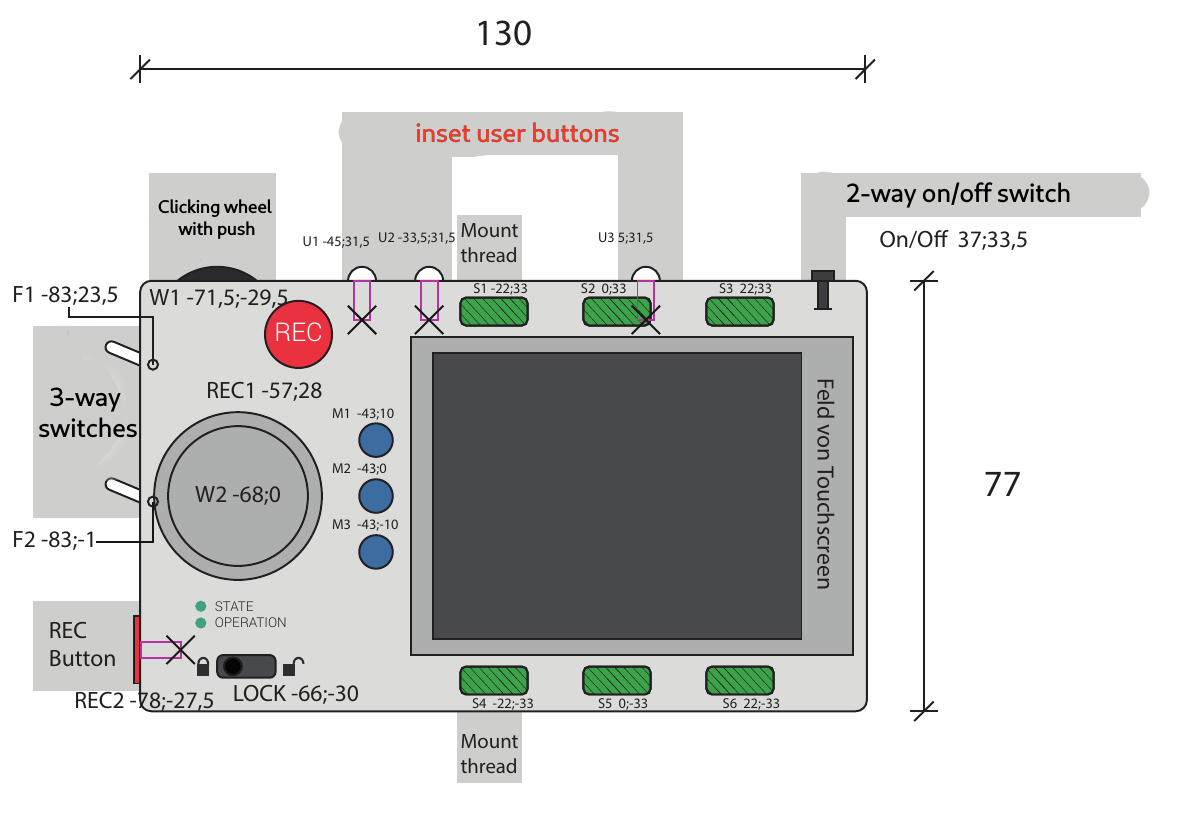
\includegraphics[width=0.8\linewidth]{images/axiom_remote_bottonPos.png}
		    \caption{AXIOM Remote Button Positions}
		    \label{fig:logo}
		\end{figure}
	\end{center}
\end{frame}

\subsection{Operation}

\begin{frame}{Operation}
	\begin{center}
		\begin{figure}[h]
		    \centering
		    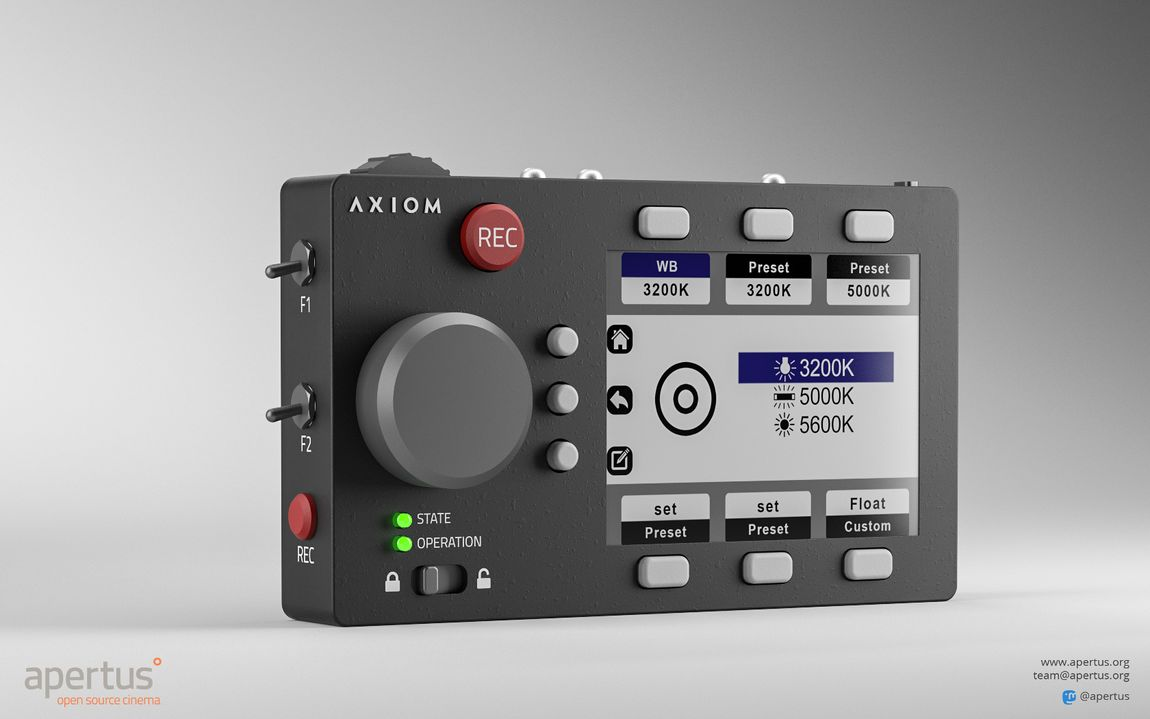
\includegraphics[width=0.8\linewidth]{images/Axiom_Remote_V3.jpg}
		    \caption{AXIOM Remote}
		    \label{fig:logo}
		\end{figure}
	\end{center}
\end{frame}


\begin{frame}{Operation (Cont.)}
	\begin{itemize}
		\item Six buttons - to select the options
		\item Currently in the new design - only "home" and "back" buttons are present
		\item In the older version - there are left/right buttons to change the pages, a page number button to goto a particular page and for the menu items which are not self-explanatory there is a "?" (help) button
	\end{itemize}
\end{frame}

\subsection{Hardware}

\begin{frame}{Hardware}
	\begin{itemize}
		\item PCB Version 2 Prototype
		\begin{itemize}
			\item The second knob is removed
			\item Remove left side rocker switches
			\item Remove top side pushbuttons
			\item Having one white LED per pushbutton
			\item 4 more holes to PCB
			\item Replace slide switches for ON/OFF and LOCK with pushbuttons
		\end{itemize}
	\end{itemize}
\end{frame}

\begin{frame}{Hardware (Cont.)}
	\begin{center}
		\begin{figure}[h]
		    \centering
		    \includegraphics[width=0.8\linewidth]{images/Axiom_Remote_PCB.jpg}
		    \caption{PCB}
		    \label{fig:logo}
		\end{figure}
	\end{center}
\end{frame}

\subsection{Electronics}

\begin{frame}{Electronics}
	\begin{itemize}
		\item PIC32MZ was chosen as core processor, two PIC16 are used for handling push button, rotary encoder and LED IO
		\item 2.8" 320x240 TFT from Adafruit as a display
		\item USB-C Connector
		\item Currently powered externally via 5V DC supply
		\item The firmware is programmed with a PICkit2 directly into the flash memory
	\end{itemize}
\end{frame}

\subsection{GUI}

\begin{frame}{GUI}
	\begin{center}
		\begin{figure}[htbp]
		    \centering
		    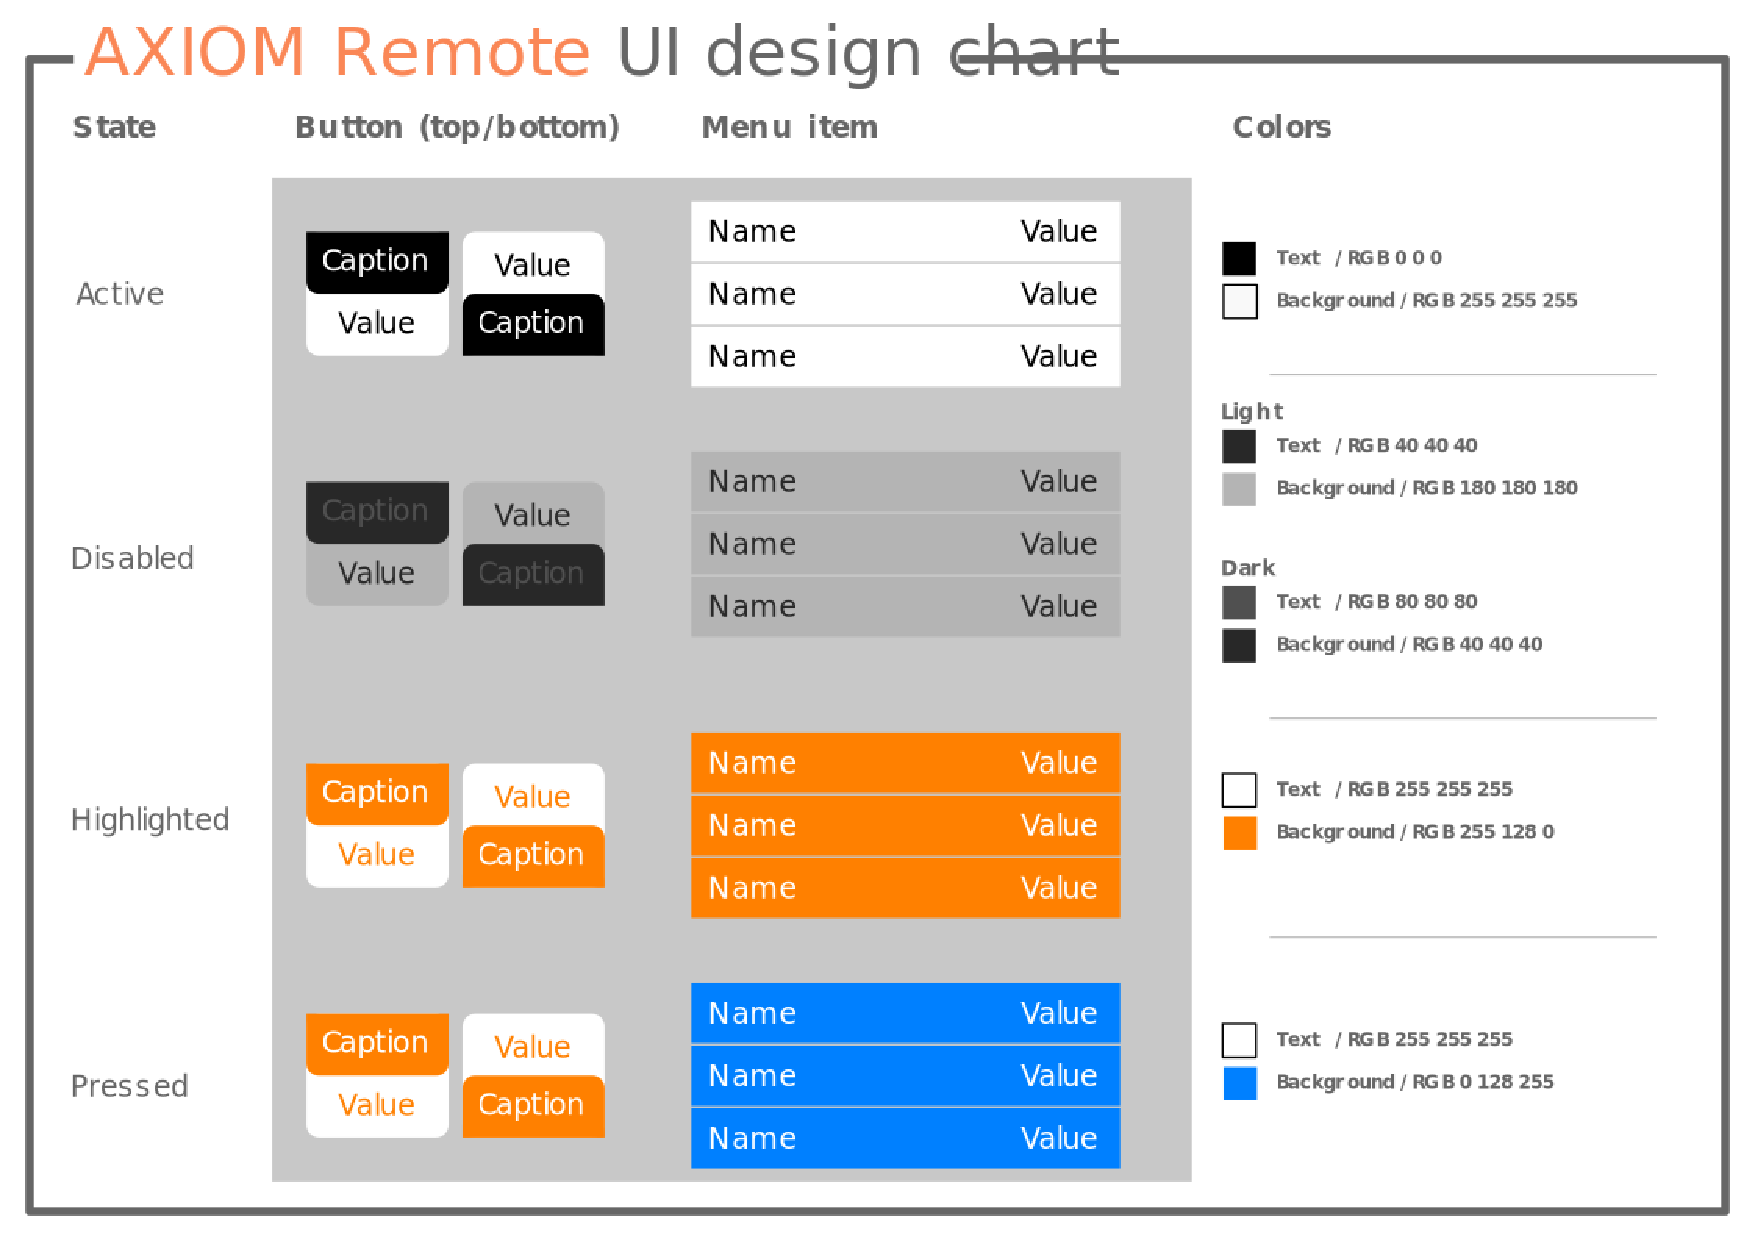
\includegraphics[width=0.7\textwidth,clip]{images/AXIOM_Remote_UI_design_chart.pdf}
		    \caption{Color Scheme}
		    \label{fig:logo}
		\end{figure}
	\end{center}
\end{frame}

\end{document}
